%% NEW 2026-10-15. The campaign in one figure: what the host path looked like as
%% first built, and what it looks like now. Everything here is measured; the
%% numbers are in Tab.~\ref{tab:ledger} and App.~\ref{app:ridercost}.
\begin{figure*}[t]
\centering
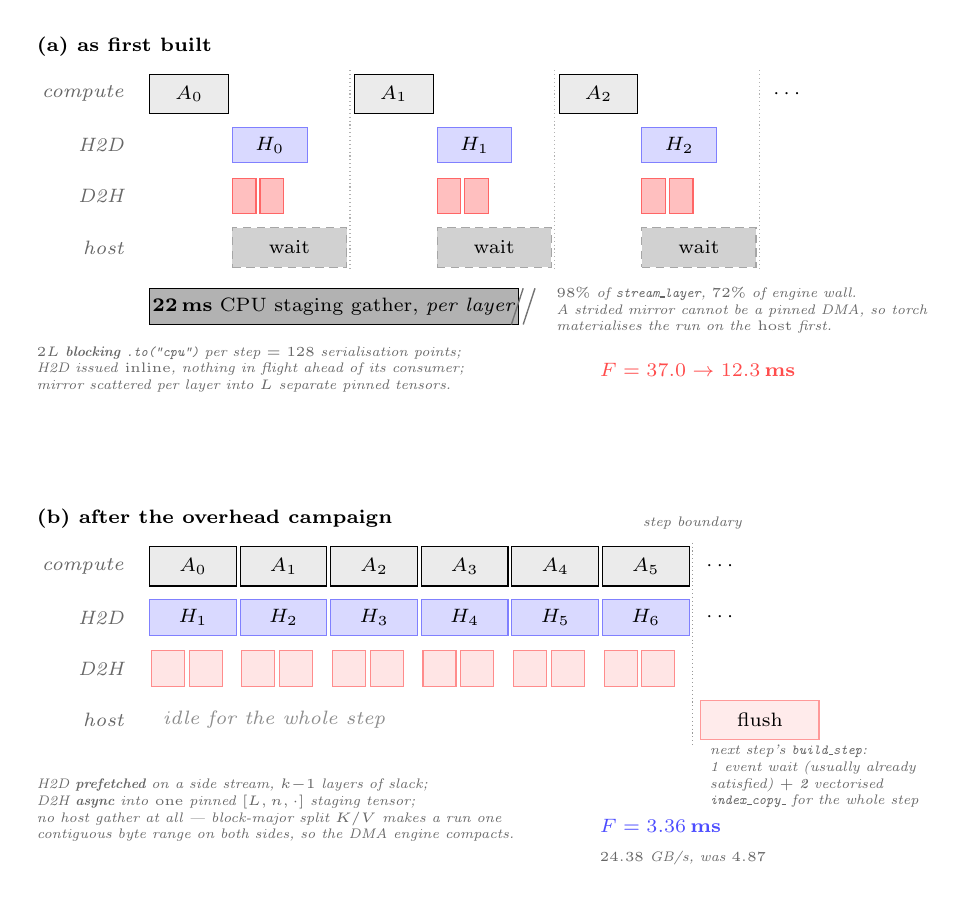
\begin{tikzpicture}[
  x=1cm, y=1cm, font=\scriptsize,
  cmp/.style={draw, fill=black!8, minimum height=5mm, inner sep=1pt},
  xfer/.style={draw, fill=blue!15, draw=blue!50, minimum height=4.5mm, inner sep=1pt},
  d2hb/.style={draw, fill=red!25, draw=red!60, minimum height=4.5mm, inner sep=0pt},
  d2ha/.style={draw, fill=red!10, draw=red!45, minimum height=4.5mm, inner sep=0pt},
  wait/.style={draw=black!35, fill=black!18, minimum height=5mm, inner sep=0pt,
               densely dashed},
  gath/.style={draw, fill=black!30, minimum height=4.5mm, inner sep=1pt},
  row/.style={font=\scriptsize\itshape, text=black!60, anchor=east},
  tag/.style={font=\scriptsize\bfseries},
  note/.style={font=\tiny\itshape, text=black!60, align=left},
]

%% ===================== (a) BASE =====================================
\node[tag, anchor=west] at (-1.55,2.55) {(a) as first built};

\node[row] at (-0.2,1.95) {compute};
\node[row] at (-0.2,1.30) {H2D};
\node[row] at (-0.2,0.65) {D2H};
\node[row] at (-0.2,0.00) {host};

%% layer 0 .. 2, each layer is 2.6cm wide because the host blocks between them
\foreach \i/\x in {0/0, 1/2.6, 2/5.2} {
  \node[cmp, minimum width=1.0cm, anchor=west] at (\x,1.95) {$A_\i$};
  \node[xfer, minimum width=0.95cm, anchor=west] at (\x+1.05,1.30) {$H_\i$};
  \node[d2hb, minimum width=0.30cm, anchor=west] at (\x+1.05,0.65) {};
  \node[d2hb, minimum width=0.30cm, anchor=west] at (\x+1.40,0.65) {};
  \node[wait, minimum width=1.45cm, anchor=west] at (\x+1.05,0.00) {wait};
  \draw[densely dotted, black!30] (\x+2.55,2.25) -- (\x+2.55,-0.3);
}
\node[anchor=west, font=\scriptsize] at (7.8,1.95) {$\cdots$};

%% the host gather, drawn clipped because it is 16x the whole rest of the row
\node[gath, minimum width=4.55cm, anchor=west] at (0,-0.75)
     {\textbf{22\,ms} CPU staging gather, \emph{per layer}};
\draw[black!55, line width=0.5pt]
      (4.60,-0.98) -- (4.75,-0.52) (4.75,-0.98) -- (4.90,-0.52);
\node[note, anchor=west] at (5.05,-0.80)
     {$98\%$ of \texttt{stream\_layer}, $72\%$ of engine wall.\\
      A strided mirror cannot be a pinned DMA, so torch\\
      materialises the run on the \emph{host} first.};

\node[note, anchor=west] at (-1.55,-1.55)
     {$2L$ \textbf{blocking} \texttt{.to("cpu")} per step $=128$ serialisation points;\\
      H2D issued \emph{inline}, nothing in flight ahead of its consumer;\\
      mirror scattered per layer into $L$ separate pinned tensors.};
\node[tag, anchor=west, text=red!70] at (5.6,-1.55) {$F=37.0\rightarrow12.3$\,ms};

%% ===================== (b) OPTIMISED ================================
\begin{scope}[yshift=-6.0cm]
\node[tag, anchor=west] at (-1.55,2.55) {(b) after the overhead campaign};

\node[row] at (-0.2,1.95) {compute};
\node[row] at (-0.2,1.30) {H2D};
\node[row] at (-0.2,0.65) {D2H};
\node[row] at (-0.2,0.00) {host};

\foreach \i/\x in {0/0, 1/1.15, 2/2.30, 3/3.45, 4/4.60, 5/5.75} {
  \node[cmp, minimum width=1.10cm, anchor=west] at (\x,1.95) {$A_\i$};
  \node[d2ha, minimum width=0.42cm, anchor=west] at (\x+0.02,0.65) {};
  \node[d2ha, minimum width=0.42cm, anchor=west] at (\x+0.50,0.65) {};
}
%% H2D is prefetched: layer l+1's transfer rides under layer l's compute
\foreach \i/\x in {1/0, 2/1.15, 3/2.30, 4/3.45, 5/4.60, 6/5.75}
  \node[xfer, minimum width=1.10cm, anchor=west] at (\x,1.30) {$H_\i$};

\node[anchor=west, font=\scriptsize] at (6.95,1.95) {$\cdots$};
\node[anchor=west, font=\scriptsize] at (6.95,1.30) {$\cdots$};

\node[anchor=west, font=\scriptsize\itshape, text=black!45] at (0.05,0.0)
     {idle for the whole step};

%% the deferred flush, at the NEXT step's boundary
\draw[densely dotted, black!40] (6.90,2.25) -- (6.90,-0.35);
\node[cmp, minimum width=1.5cm, anchor=west, fill=red!8, draw=red!40]
     at (7.0,0.0) {flush};
\node[note, anchor=west] at (7.0,-0.72)
     {next step's \texttt{build\_step}:\\
      1 event wait (usually already\\
      satisfied) $+$ \textbf{2} vectorised\\
      \texttt{index\_copy\_} for the whole step};
\node[note, anchor=south] at (6.90,2.30) {step boundary};

\node[note, anchor=west] at (-1.55,-1.15)
     {H2D \textbf{prefetched} on a side stream, $k{-}1$ layers of slack;\\
      D2H \textbf{async} into \emph{one} pinned $[L,n,\cdot]$ staging tensor;\\
      no host gather at all --- block-major split $K/V$ makes a run one\\
      contiguous byte range on both sides, so the DMA engine compacts.};
\node[tag, anchor=west, text=blue!70] at (5.6,-1.35) {$F=3.36$\,ms};
\node[note, anchor=west] at (5.6,-1.75) {$24.38$ GB/s, was $4.87$};
\end{scope}

\end{tikzpicture}
\caption{\textbf{The host path as first built (a) and after the overhead campaign
(b).} Three changes do the work. The transfer moves from \emph{inline} to
\emph{prefetched}, so layer $\ell{+}1$'s refresh is in flight while layer $\ell$
computes. The token write-back moves from $2L$ blocking copies per step --- $128$
points at which the host waits on the device --- to $2L$ asynchronous copies into a
single staging tensor, drained once at the next step's boundary. And the host-side
staging gather, which dominated everything else and which a faster interconnect
would not have touched, is eliminated outright by making a run contiguous on both
sides. Bar widths are schematic; all quoted figures are measured.}
\label{fig:basevsopt}
\end{figure*}
